
% !TEX encoding = UTF-8 Unicode



  \documentclass[conference,compsoc]{IEEEtran}
  % Some/most Computer Society conferences require the compsoc mode option,
  % but others may want the standard conference format.
  %
  % If IEEEtran.cls has not been installed into the LaTeX system files,
  % manually specify the path to it like:
  % \documentclass[conference,compsoc]{../sty/IEEEtran}

  \usepackage{graphicx}
  \usepackage{epstopdf}
  \DeclareGraphicsExtensions{.eps}
  \usepackage{url}
  \usepackage{multicol}% http://ctan.org/pkg/multicols



\usepackage{graphicx}
\usepackage{epstopdf}
\DeclareGraphicsExtensions{.eps}
\usepackage{url}
\usepackage{multicol}% http://ctan.org/pkg/multicols
\usepackage{epigraph}
\setlength{\epigraphwidth}{.85\textwidth}

\usepackage[utf8x]{inputenc} 

\usepackage{array}
\newcolumntype{L}[1]{>{\raggedright\let\newline\\\arraybackslash\hspace{0pt}}m{#1}}
\newcolumntype{C}[1]{>{\centering\let\newline\\\arraybackslash\hspace{0pt}}m{#1}}
\newcolumntype{R}[1]{>{\raggedleft\let\newline\\\arraybackslash\hspace{0pt}}m{#1}}
\usepackage{subcaption}
\usepackage[utf8]{inputenc}
\usepackage[portuguese]{babel}
\usepackage{listings,mdframed}

\usepackage{textcomp}
\usepackage{hyperref}



  % *** CITATION PACKAGES ***
  %
  \ifCLASSOPTIONcompsoc
  % IEEE Computer Society needs nocompress option
% requires cite.sty v4.0 or later (November 2003)
  \usepackage[nocompress]{cite}
  \else
  % normal IEEE
  \usepackage{cite}
  \fi
  

  % *** GRAPHICS RELATED PACKAGES ***
  %
  \ifCLASSINFOpdf
  % \usepackage[pdftex]{graphicx}
  % declare the path(s) where your graphic files are
  % \graphicspath{{../pdf/}{../jpeg/}}
  % and their extensions so you won't have to specify these with
  % every instance of \includegraphics
  % \DeclareGraphicsExtensions{.pdf,.jpeg,.png}
  \else
  % or other class option (dvipsone, dvipdf, if not using dvips). graphicx
  % will default to the driver specified in the system graphics.cfg if no
  % driver is specified.
  % \usepackage[dvips]{graphicx}
  % declare the path(s) where your graphic files are
  % \graphicspath{{../eps/}}
  % and their extensions so you won't have to specify these with
  % every instance of \includegraphics
  % \DeclareGraphicsExtensions{.eps}
  \fi
  
  % correct bad hyphenation here
  \hyphenation{op-tical net-works semi-conduc-tor}

  \usepackage[utf8x]{inputenc} 

  \usepackage{array}
  \newcolumntype{L}[1]{>{\raggedright\let\newline\\\arraybackslash\hspace{0pt}}m{#1}}
  \newcolumntype{C}[1]{>{\centering\let\newline\\\arraybackslash\hspace{0pt}}m{#1}}
  \newcolumntype{R}[1]{>{\raggedleft\let\newline\\\arraybackslash\hspace{0pt}}m{#1}}


\usepackage{float}
\usepackage{listings}

\lstdefinestyle{esc} {
language=c,
	keywordstyle=\bfseries\ttfamily\color[rgb]{0,0,1},
	identifierstyle=\ttfamily,
	commentstyle=\color[rgb]{0.133,0.545,0.133},
	stringstyle=\ttfamily\color[rgb]{0.627,0.126,0.941},
	showstringspaces=false,
	basicstyle=\tiny,
numberstyle=\small,
numbers=right,
	stepnumber=1,
	numbersep=10pt,
	tabsize=1,
	breaklines=true,
	prebreak = \raisebox{0ex}[0ex][0ex]{\ensuremath{\hookleftarrow}},
	breakatwhitespace=false,
	%aboveskip={1.5\baselineskip},
  columns=fixed,
  upquote=true,
  extendedchars=true,
 frame=single,
}

\lstdefinestyle{command}{
backgroundcolor=\color{yellow},frame=shadowbox,
language=c,
	keywordstyle=\bfseries\ttfamily\color[rgb]{0,0,1},
	identifierstyle=\ttfamily,
	commentstyle=\color[rgb]{0.133,0.545,0.133},
	stringstyle=\ttfamily\color[rgb]{0.627,0.126,0.941},
	showstringspaces=false,
	basicstyle=\scriptsize,
numberstyle=\small,
numbers=right,
	stepnumber=1,
	numbersep=10pt,
	tabsize=1,
	breaklines=true,
	prebreak = \raisebox{0ex}[0ex][0ex]{\ensuremath{\hookleftarrow}},
	breakatwhitespace=false,
	%aboveskip={1.5\baselineskip},
  columns=fixed,
  upquote=true,
  extendedchars=true,
}

\lstset{
	language=c,
	keywordstyle=\bfseries\ttfamily\color[rgb]{0,0,1},
	identifierstyle=\ttfamily,
	commentstyle=\color[rgb]{0.133,0.545,0.133},
	stringstyle=\ttfamily\color[rgb]{0.627,0.126,0.941},
	showstringspaces=false,
	basicstyle=\scriptsize,
numberstyle=\small,
numbers=right,
	stepnumber=1,
	numbersep=10pt,
	tabsize=1,
	breaklines=true,
	prebreak = \raisebox{0ex}[0ex][0ex]{\ensuremath{\hookleftarrow}},
	breakatwhitespace=false,
	%aboveskip={1.5\baselineskip},
  columns=fixed,
  upquote=true,
  extendedchars=true,
 frame=single
 %backgroundcolor=\color{lbcolor},
}


  \begin{document}
  %
  % paper title
  % Titles are generally capitalized except for words such as a, an, and, as,
  % at, but, by, for, in, nor, of, on, or, the, to and up, which are usually
  % not capitalized unless they are the first or last word of the title.
  % Linebreaks \\ can be used within to get better formatting as desired.
  % Do not put math or special symbols in the title.
  \title{Introdução ao PERF\\ Determinação de Hotspots de execução de kernels recorrendo a PERF (linux-tools)}

  % author names and affiliations
  % use a multiple column layout for up to three different
  % affiliations
  \author{\IEEEauthorblockN{Filipe Oliveira}
    \IEEEauthorblockA{Departamento de Informática\\
      Universidade do Minho\\
        Email: a57816@alunos.uminho.pt}
  }

% conference papers do not typically use \thanks and this command
% is locked out in conference mode. If really needed, such as for
% the acknowledgment of grants, issue a \IEEEoverridecommandlockouts
% after \documentclass

% for over three affiliations, or if they all won't fit within the width
% of the page (and note that there is less available width in this regard for
    % compsoc conferences compared to traditional conferences), use this
% alternative format:
% 
%\author{\IEEEauthorblockN{Michael Shell\IEEEauthorrefmark{1},
  %Homer Simpson\IEEEauthorrefmark{2},
  %James Kirk\IEEEauthorrefmark{3}, 
  %Montgomery Scott\IEEEauthorrefmark{3} and
    %Eldon Tyrell\IEEEauthorrefmark{4}}
  %\IEEEauthorblockA{\IEEEauthorrefmark{1}School of Electrical and Computer Engineering\\
    %Georgia Institute of Technology,
  %Atlanta, Georgia 30332--0250\\ Email: see http://www.michaelshell.org/contact.html}
  %\IEEEauthorblockA{\IEEEauthorrefmark{2}Twentieth Century Fox, Springfield, USA\\
    %Email: homer@thesimpsons.com}
  %\IEEEauthorblockA{\IEEEauthorrefmark{3}Starfleet Academy, San Francisco, California 96678-2391\\
    %Telephone: (800) 555--1212, Fax: (888) 555--1212}
  %\IEEEauthorblockA{\IEEEauthorrefmark{4}Tyrell Inc., 123 Replicant Street, Los Angeles, California 90210--4321}}




  % use for special paper notices
  %\IEEEspecialpapernotice{(Invited Paper)}




  % make the title area
  \maketitle

  % As a general rule, do not put math, special symbols or citations
  % in the abstract
  %\begin{abstract}

  %Neste estudo, analisamos a performance de kernels 
  %\end{abstract}

  % no keywords




  % For peer review papers, you can put extra information on the cover
  % page as needed:
  % \ifCLASSOPTIONpeerreview
  % \begin{center} \bfseries EDICS Category: 3-BBND \end{center}
  % \fi
  %
  % For peerreview papers, this IEEEtran command inserts a page break and
  % creates the second title. It will be ignored for other modes.
  \IEEEpeerreviewmaketitle



  %\section{Introduction}
  % no \IEEEPARstart
  %This demo file is intended to serve as a ``starter file''
  %for IEEE Computer Society conference papers produced under \LaTeX\ using
  %IEEEtran.cls version 1.8b and later.
  % You must have at least 2 lines in the paragraph with the drop letter
% (should never be an issue)
  %I wish you the best of success.

  %\hfill Filipe Oliveira

  %\hfill 1 Março, 2016

  \section{Introdução -- Contextualização da utilização da ferramenta PERF}  
  
O presente trabalho prático surge como um "diário de bordo" relativo ao acompanhamento de um conjunto de 3 parte do tutorual: \textbf{"PERF tutorial: Finding execution hot spots"}.\footnote{\url{http://sandsoftwaresound.net/perf/perf-tutorial-hot-spots/}}
\par 
A parte 1 descreve a utilização da ferramenta PERF como meio de identificação e análise de hotspots de execução em kernels. Cobre maioritariamente os comandos PERF mais básico, e respectivas opções e eventos de medição de performance relativa.\par 
A parte 2 introduz eventos que permitem a medição de contadores de hardware e demonstra a utilização do PERF nesse sentido. Discute ainda a importância de certas métricas de performance e a sua influência relativa na performance geral de uma aplicação.\par 
A parte 3 recorre aos eventos de contadores de hardware para, uma vez mais e desta vez de uma forma mais aprofundada, analisar os hotspots de um kernel/aplicação.\par 
Todo o tutorial assenta em duas versões de uma aplicação de multiplicação de matrizes:
begin{itemize}
\item \textbf{Naive:} Algoritmo de multiplicação de matrizes com acessos a memória "column-wise". 
\item \textbf{Interchange:}  Algoritmo de multiplicação de matrizes com acessos a memória "row-wise". 
\end{itemize}
A primeira versão serão, com seria de esperar, apresentará problemas de performance relacionados com o acesso à memória. É importante também realçar que as aplicações são ambas compiladas com a versão de compilador GCC 4.9.0., com as seguintes flags de compilação "-O2 -ggdb -g". Denote que a flag de otimização -O3, que activa um conjunto de otimizações de código\footnote{-finline-functions, -funswitch-loops, -fpredictive-commoning, -fgcse-after-reload, -ftree-vectorize, -fvect-cost-model, -ftree-partial-pre and -fipa-cp-clone options} está desativada, muito pela necessidade de manter o código (apesar de pouco eficiente) legível e com capacidade de ser compreendido pelo programador.\par 


  \section{Caracterização do Hardware do ambiente de testes}
  
  Tão importante com especificar as versões de código e as propriedades é especificar os ambientes de teste nos quais pretendemos realizar as benchmarks. \par 
  Através da análise do hardware disponível no Search6 \footnote{Services and Advanced Research Computing with HTC/HPC clusters}, uma das nossas plataformas de teste, foi seleccionado o nó do tipo compute-431, sendo a disponibilidade global do mesmo e o correcto funcionamento do perf os principais factores. Na tabela \ref{table:characterization_431} encontram-se especificadas as principais características dos sistemas em teste.\par 

  \begin{table}[H]
  \caption{Características de Hardware do nó 431}
  \label{table:characterization_431}
  \centering
  \begin{tabular}{ | l | r | }

  \hline
  Sistema & compute-431 \\ \hline \hline
  \# CPUs & 2  \\ \hline
  CPU & Intel\textsuperscript{\textregistered} Xeon\textsuperscript{\textregistered} X5650 \\ \hline 
  Arquitectura de Processador & Nehalem  \\ \hline 
  \# Cores por CPU & 6   \\ \hline 
  \# Threads por CPU & 12  \\ \hline 
  Freq. Clock & 2.66 GHz  \\ \hline
  Cache L1  & 192KB  (32KB por Core)  \\ \hline 
  Cache L2  & 1536KB (256KB por Core)  \\ \hline 
  Cache L3  & 12288KB (partilhada) \\ \hline 
  Ext. Inst. Set  & SSE4.2   \\ \hline 
  \#Memory Channels & 3 \\ \hline
  Memória Ram Disponível & 48GB \\ \hline
  Peak Memory BW Fab. CPU  & 32 GB/s \\ \hline
	
  \end{tabular}
  \end{table}

  \section{Determinação do tamanho dos datasets}

Talvez dos pontos mais importantes presente na tabela de caracterização de hardware seja o tamanho da Cache L3, dado que ambos os algoritmos dependem massivamente de leitura/escrita na memória principal. Assim sendo, se pretendemos realçar as penalizações resultantes de diferentes tipos de acesso aos dados devemos realizar dois tipos distintos de testes:
\begin{itemize}
\item Matrizes contidas na LLC: \par Sabemos que as 3 matrizes terão de ter uma tamanho de coluna/linha inferior a: \[lado\ matriz \leq \frac{\sqrt{(\frac{12288KB}{4\ Bytes\ p/ float}}}{3\ matrizes} \leq 1011\] para que os datasets estejam completamente contidos em cache. Foi escolhido o lado da matriz de 512 elementos.
\item Matrizes contidas na memória principal: \par 
Sabemos que as 3 matrizes terão de ter uma tamanho de coluna/linha superior a 1011 elemento por linha/coluna. Foi escolhido o lado da matriz de 2048 elementos.\par
Dorante, todos os comandos apresentados terão por standard o dataset menor (matrizes de 512*512), e o kernel naive. Em caso de serem utilizados outro kernel ou dataset será feita a referência antes da apresentação dos resultados.
\section{Parte 1 }

\subsection{Passo 0 -- uma análise aos software e hardware events disponíveis na máquina}
Recorrendo ao seguinte commando:
 \begin{lstlisting}[style=command]
[a57816@compute-431-1 ESC_FLAME_GRAPH]$ perf list | wc -l   
\end{lstlisting}
Podemos ter uma noção em ternos de eventos de hardware e software disponíveis na máquina de teste:
\begin{lstlisting}
784
\end{lstlisting}
   
\subsection{1º Passo -- o encontrar dos tempos base sem overhead de medição para o menor dataset (dataset em LLCACHE)}

Por forma 	a podermos estabelecer um limite dentro do aceitável das possíveis alterações à performance das versões do kernel necessitamos de primeiramente ter uma medição com o mínimo de overhead possível, para o menor dataset em profiling (matriz 512*512), para o caso \textbf{naive}. Recorrendo ao seguinte comando:

 \begin{lstlisting}[style=command]
[a57816@compute-431-1 ESC_FLAME_GRAPH]$ perf stat -e cpu-clock ./naive
   \end{lstlisting}
\begin{lstlisting}
 Performance counter stats for './naive':

        201.696023      cpu-clock (msec)                                            

       0.206153405 seconds time elapsed
\end{lstlisting}
Teremos uma base de referência futura, para podermos validar as nossas medições com overhead.\par 
Para além do tempo de execução é ainda demonstrado o número de cpu-clocks necessários para a execução.\par  

Como seria de esperar, é possível num única medição registar vários eventos. Recorrendo ao seguinte comando:

 \begin{lstlisting}[style=command]
[a57816@compute-431-1 ESC_FLAME_GRAPH]$ perf stat -e cpu-clock,faults ./naive
   \end{lstlisting}
\lstinputlisting[language=C]{../2_naive_cpu_clock_faults.txt} %input de um ficheiro

\subsection{O processo de procura de hotpsots de uma aplicação}       

O processo de procura de hotpsots de uma aplicação pode ser traduzido em 2 passos simples:
\begin{itemize}
\item Passo 1: Recolha de dados para profiling da aplicação
\item Passo 2 : Tratamento e apresentação da informação recolhida.
\end{itemize}
    
\subsubsection{Passo 1}
Podemos recolher informação de profiling simplesmente correndo o seguinte comando:
\label{passo1}
\lstinputlisting[style=command]{../3_command.txt} %input de um ficheiro

Neste caso específico o PERF corre a aplicação naive e recolhe dados relativos aos eventos: cpu-clock e page-faults. 
\lstinputlisting[language=C]{../3_step_1.txt} %input de um ficheiro


\subsubsection{Passo 2}
\par 
Relativamente ao passo 2 - Tratamento e apresentação da informação recolhida - o seguinte comando permite visualizar a informação presente no ficheiro prof.data (ficheiro default no qual é gravada a informação): \par 

\lstinputlisting[style=command]{../4_command.txt} %input de um ficheiro
\lstinputlisting[language=C]{../4_perf_report_stdio.txt} %input de um ficheiro


Existem outras alternativas a esse mesmo comando sendo esta:

\lstinputlisting[style=command]{../4_command_1.txt} %input de um ficheiro

que apresenta o Terminal-based User Interface (TUI).\par 
 Voltemos ao output apresentado pelo comando com a opção \-\-stdio. Denote no seguinte detalhe:
 
 \lstinputlisting[language=C]{../4_perf_detail.txt} %input de um ficheiro

 Como poderá confirmar foram registadas 808 medições do evento "cpu-clock".\par
 Adicionando a opção - -sort  conseguimos uma visualização agregada. Em conjunção com a opção \textbf{comm} e \textbf{dso} obtemos o seguinte resultado.
 
\lstinputlisting[style=command]{../5_command.txt} %input de um ficheiro
\lstinputlisting[language=C]{../5_report_stdio_sort.txt} %input de um ficheiro

Como pode confirmar pelo output, as duas opções no comando permitem agregar os resultados por comando e shared object.\par 

Por forma a simplificar o processo de catalogação e posterior tratamento de dados é possível aceder a metadados das medições, através da junção da opção \textbf{--header} ao comando anterior.
Desta forma temos acesso a por exemplo, os dados de hardware do ambiente de teste, o comando perf utilizado e informação relativa aos eventos medidos. Esta funcionalidade torna-se bastante útil dada a tremenda facilidade que temos hoje em dia de gerar dados de teste. A consequência da facilidade de tal geração é a posterior necessidade de tratamento correcto dos mesmos.\par 




\lstinputlisting[style=command]{../6_command.txt} %input de um ficheiro
\lstinputlisting[language=C]{../6_report_stdio_sort_header.txt} %input de um ficheiro


\subsubsection{Aumentar a granularidade do profilling -- fase I}

O exemplo dado anteriormente apresenta os dados agregados relativos a toda a aplicação. Ora, daí podemos observar que   \textbf{97.03\%} do tempo de execução é despendido em métodos da própria aplicação, enquanto que os restantes \textbf{2.48\%} são despendidos na biblioteca do sistema \textbf{libc-2.12.so}.\par 
O próximo passo será portanto aumentar a granularidade do profilling nestes dois "shared objects".

\lstinputlisting[style=command]{../7_command.txt} %input de um ficheiro
\lstinputlisting[language=C]{../7_report_stdio_dsos.txt} %input de um ficheiro

O método \textbf{multiply\_matrices()} é o responsável pela maioria do tempo de computação, sendo aproximadamente 94.86\%. \par A segunda função, em termos de tempo de computação é a \textbf{initialize\_matrices} com 2.10\%. \par 
Podemos ainda analisar as \textbf{page faults} da aplicação, sendo que a maioria ocorre no método \textbf{initialize\_matrices} -- 63.61\%, como seria de esperar. Este comportamento é o esperado, e não é responsável por qualquer problema de performance da aplicação, dado que esse mesmo método apenas ocupa 2.10\% do tempo total da aplicação, não afectando o processo de multiplicação de matrizes, que é o responsável pela maior porção do mesmo.\par 
Podemos ainda "validar" o número de page faults ocorrido, associando-o ao tamanho da matriz em uso. Ora, 512*512 floats representa um total de $512*512*(4\ bytes) = 1024KB $, multiplicado por 3 (3 matrizes), representa um total de 3072 KB, que representa um total de páginas $\frac{3072KB}{4KB\ por\ página} = 768$. Ora, 63.61\% do total de \textbf{page fauts} contabilizadas representa $0.6361 * 1157 = 735,9677 = 736\ páginas$, como espectado.

\subsubsection{Aumentar a granularidade do profilling -- fase II}
Agora que temos a completa percepção de qual o método que está a consumir maioritariamente o tempo de execução, podemos realizar um análise não por biblioteca, mas por método, associando então ao método \textbf{multiply\_matrices()} o respectivo código máquina e posição relativa ao início do método, recorrendo ao comando:

\lstinputlisting[style=command]{../8_command.txt} %input de um ficheiro

Produzindo o seguinte output: 
\lstinputlisting[language=C]{../8_annotate.txt} %input de um ficheiro

Caso pretendamos retirar o código na linguagem de alto nível, mantendo apenas a associação a código máquina com percentagem de tempo de execução, podemos recorrer ao seguinte comando:
\lstinputlisting[style=command]{../9_command.txt} %input de um ficheiro
\lstinputlisting[language=C]{../9_annotate_no_source.txt} %input de um ficheiro

Pela análise da execução dos dois comandos anteriores, temos então a resposta há muito aguardada. O nosso primeiro trabalho de detective dá-se por terminado com descoberta da  "principal responsável":

\lstinputlisting[style=command]{../9_line.txt} %input de um ficheiro

\subsection{Método de profiling}

Recolhidos os dados e descoberto o "culpado" resta-nos saber se o "modus operandi" da recursão ao comando PERF foi o mais indicado.\par
O PERF recorre a sampling estatístico para recolher os dados de profiling. Cada amostra é recolhida com base num tempo constante, tendo por base o \textbf{Linux time clock} para medir também a passagem do mesmo. Quando termina o intervalo de tempo constante é gerada uma interrupção e o PERF determina o trabalho que estava a ser realizado pelo CPU no momento da interrupção, registando por exemplo metadados do CPU, program counter, e software, produzindo aquilo que é chamado de um \textbf{sample}, sendo este escrito num buffer, posteriormente escrito no ficheiro \textbf{perf.data}. \par 

Dado que nos iremos basear no sampling estatístico para inferir conclusões acerca do comportamento de um kernel necessitamos de ser cautelosos quanto ao número de samples a recolher. \textbf{Se por um lado o excesso de amostras levará a uma interferência nos dados a serem medidos, a falta delas levará à incerteza.} Poderemos estar a concluir erradamente que uma porção de código é a responsável pela degradação de performance devido à falta de amostras que nos apontem noutro sentido. \par 

Uma forma de aumentar o número de amostras é especificando a frequência sobre a qual as mesmas serão recolhidas, através do seguinte comando: 

\lstinputlisting[style=command]{../10_command.txt} %input de um ficheiro
\lstinputlisting[language=C]{../10_freq8000.txt} %input de um ficheiro

A execução do comando anterior resultou na recolha do dobro de amostras ( 1636 amostras vs as anteriores 830) em comparação com a medição efectuada em \ref{passo1}, devido também ao aumento em dobro da frequência -- 8000 vs 4000, tal como pode ser confirmado pela execução do comando seguinte: 

\lstinputlisting[style=command]{../11_command.txt} %input de um ficheiro
\lstinputlisting[language=C]{../11_nr_samples.txt} %input de um ficheiro

Confirmamos portanto que se mantém o ponto crítico da nossa aplicação. 94.74\% do tempo da mesma foi despendido no método \textbf{multiply\_matrices}, tal como pretendíamos confirmar. 

\section{Parte 2 }

Encontrado o ponto alvo na "investigação" anterior, resta-nos resolver o problema. Atente nas seguintes transcrições de código, pertencentes nomeadamente à versão naive e interchange:
\begin{itemize}
\item{ Naive: \par \lstinputlisting[language=C]{../11_5_naive_detail.c} %input de um ficheiro
Ilustração do acesso às posições da matriz via ordem IJK:\par 
      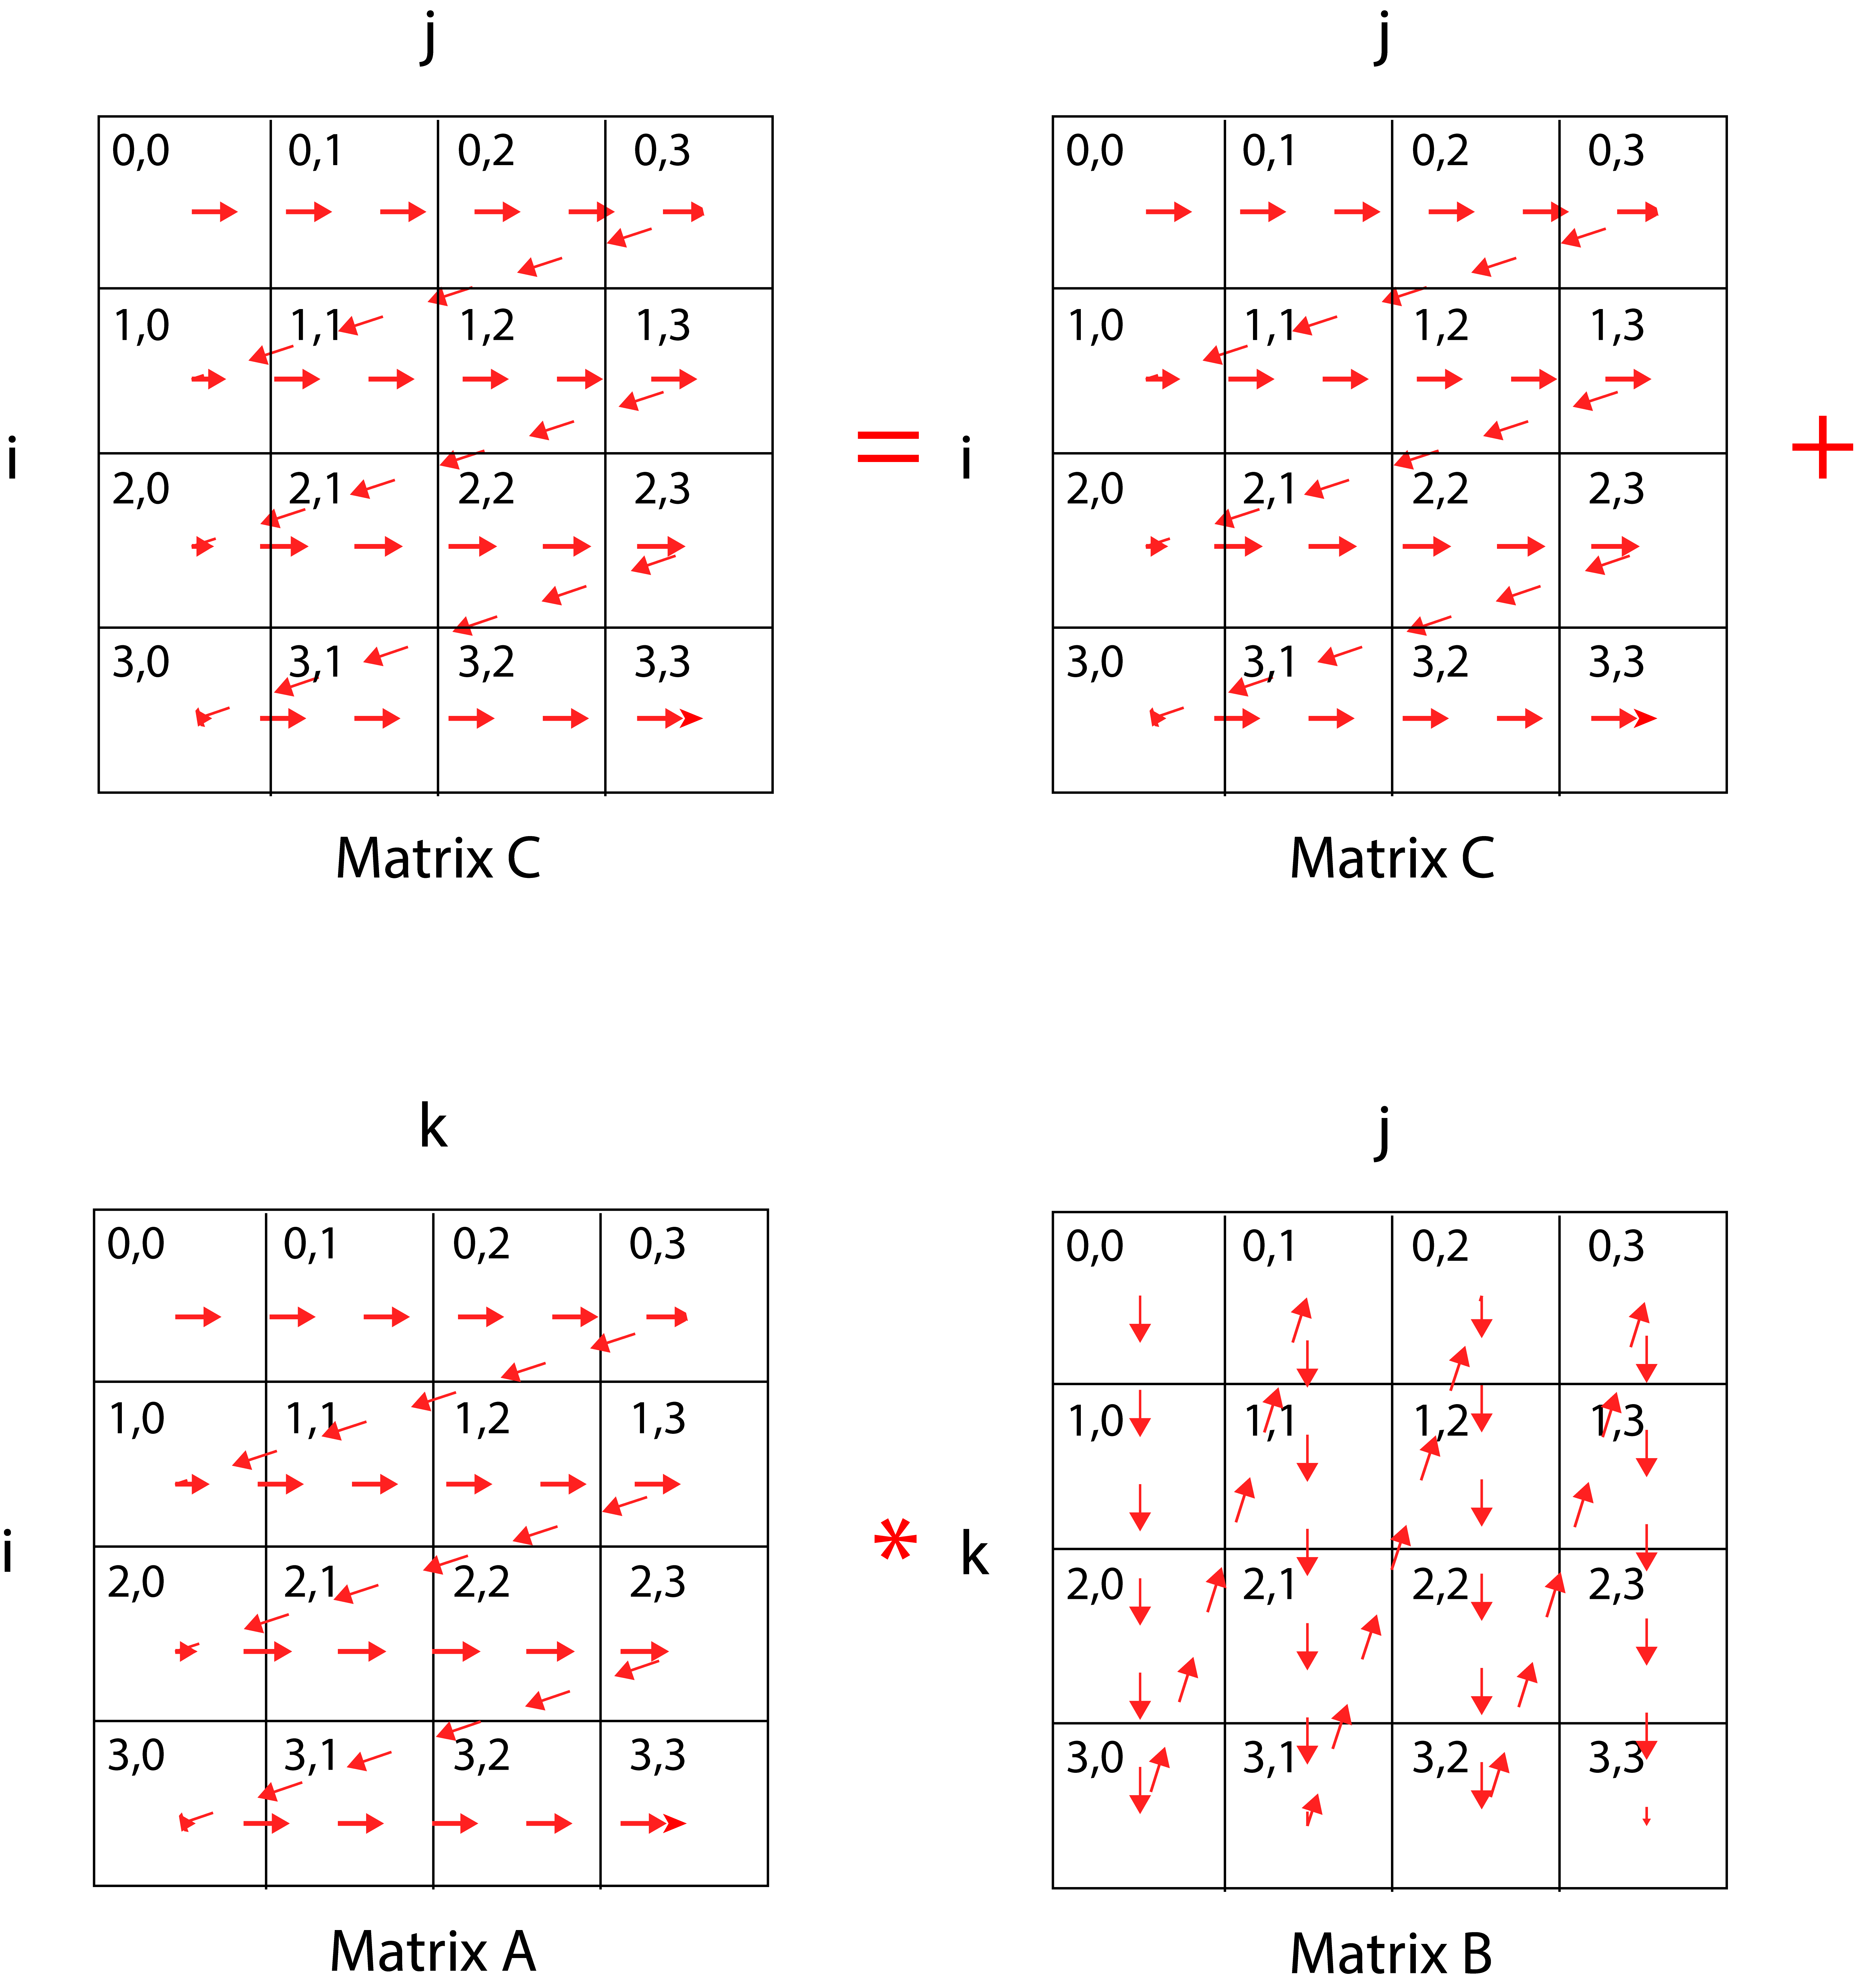
\includegraphics[width=0.75\columnwidth]{PNG/matrix_ijk_final.png}
      

\item {Interchage: \par  \lstinputlisting[language=C]{../11_5_interchage_detail.c} %input de um ficheiro
Ilustração do acesso às posições da matriz via ordem IKJ:\par 
      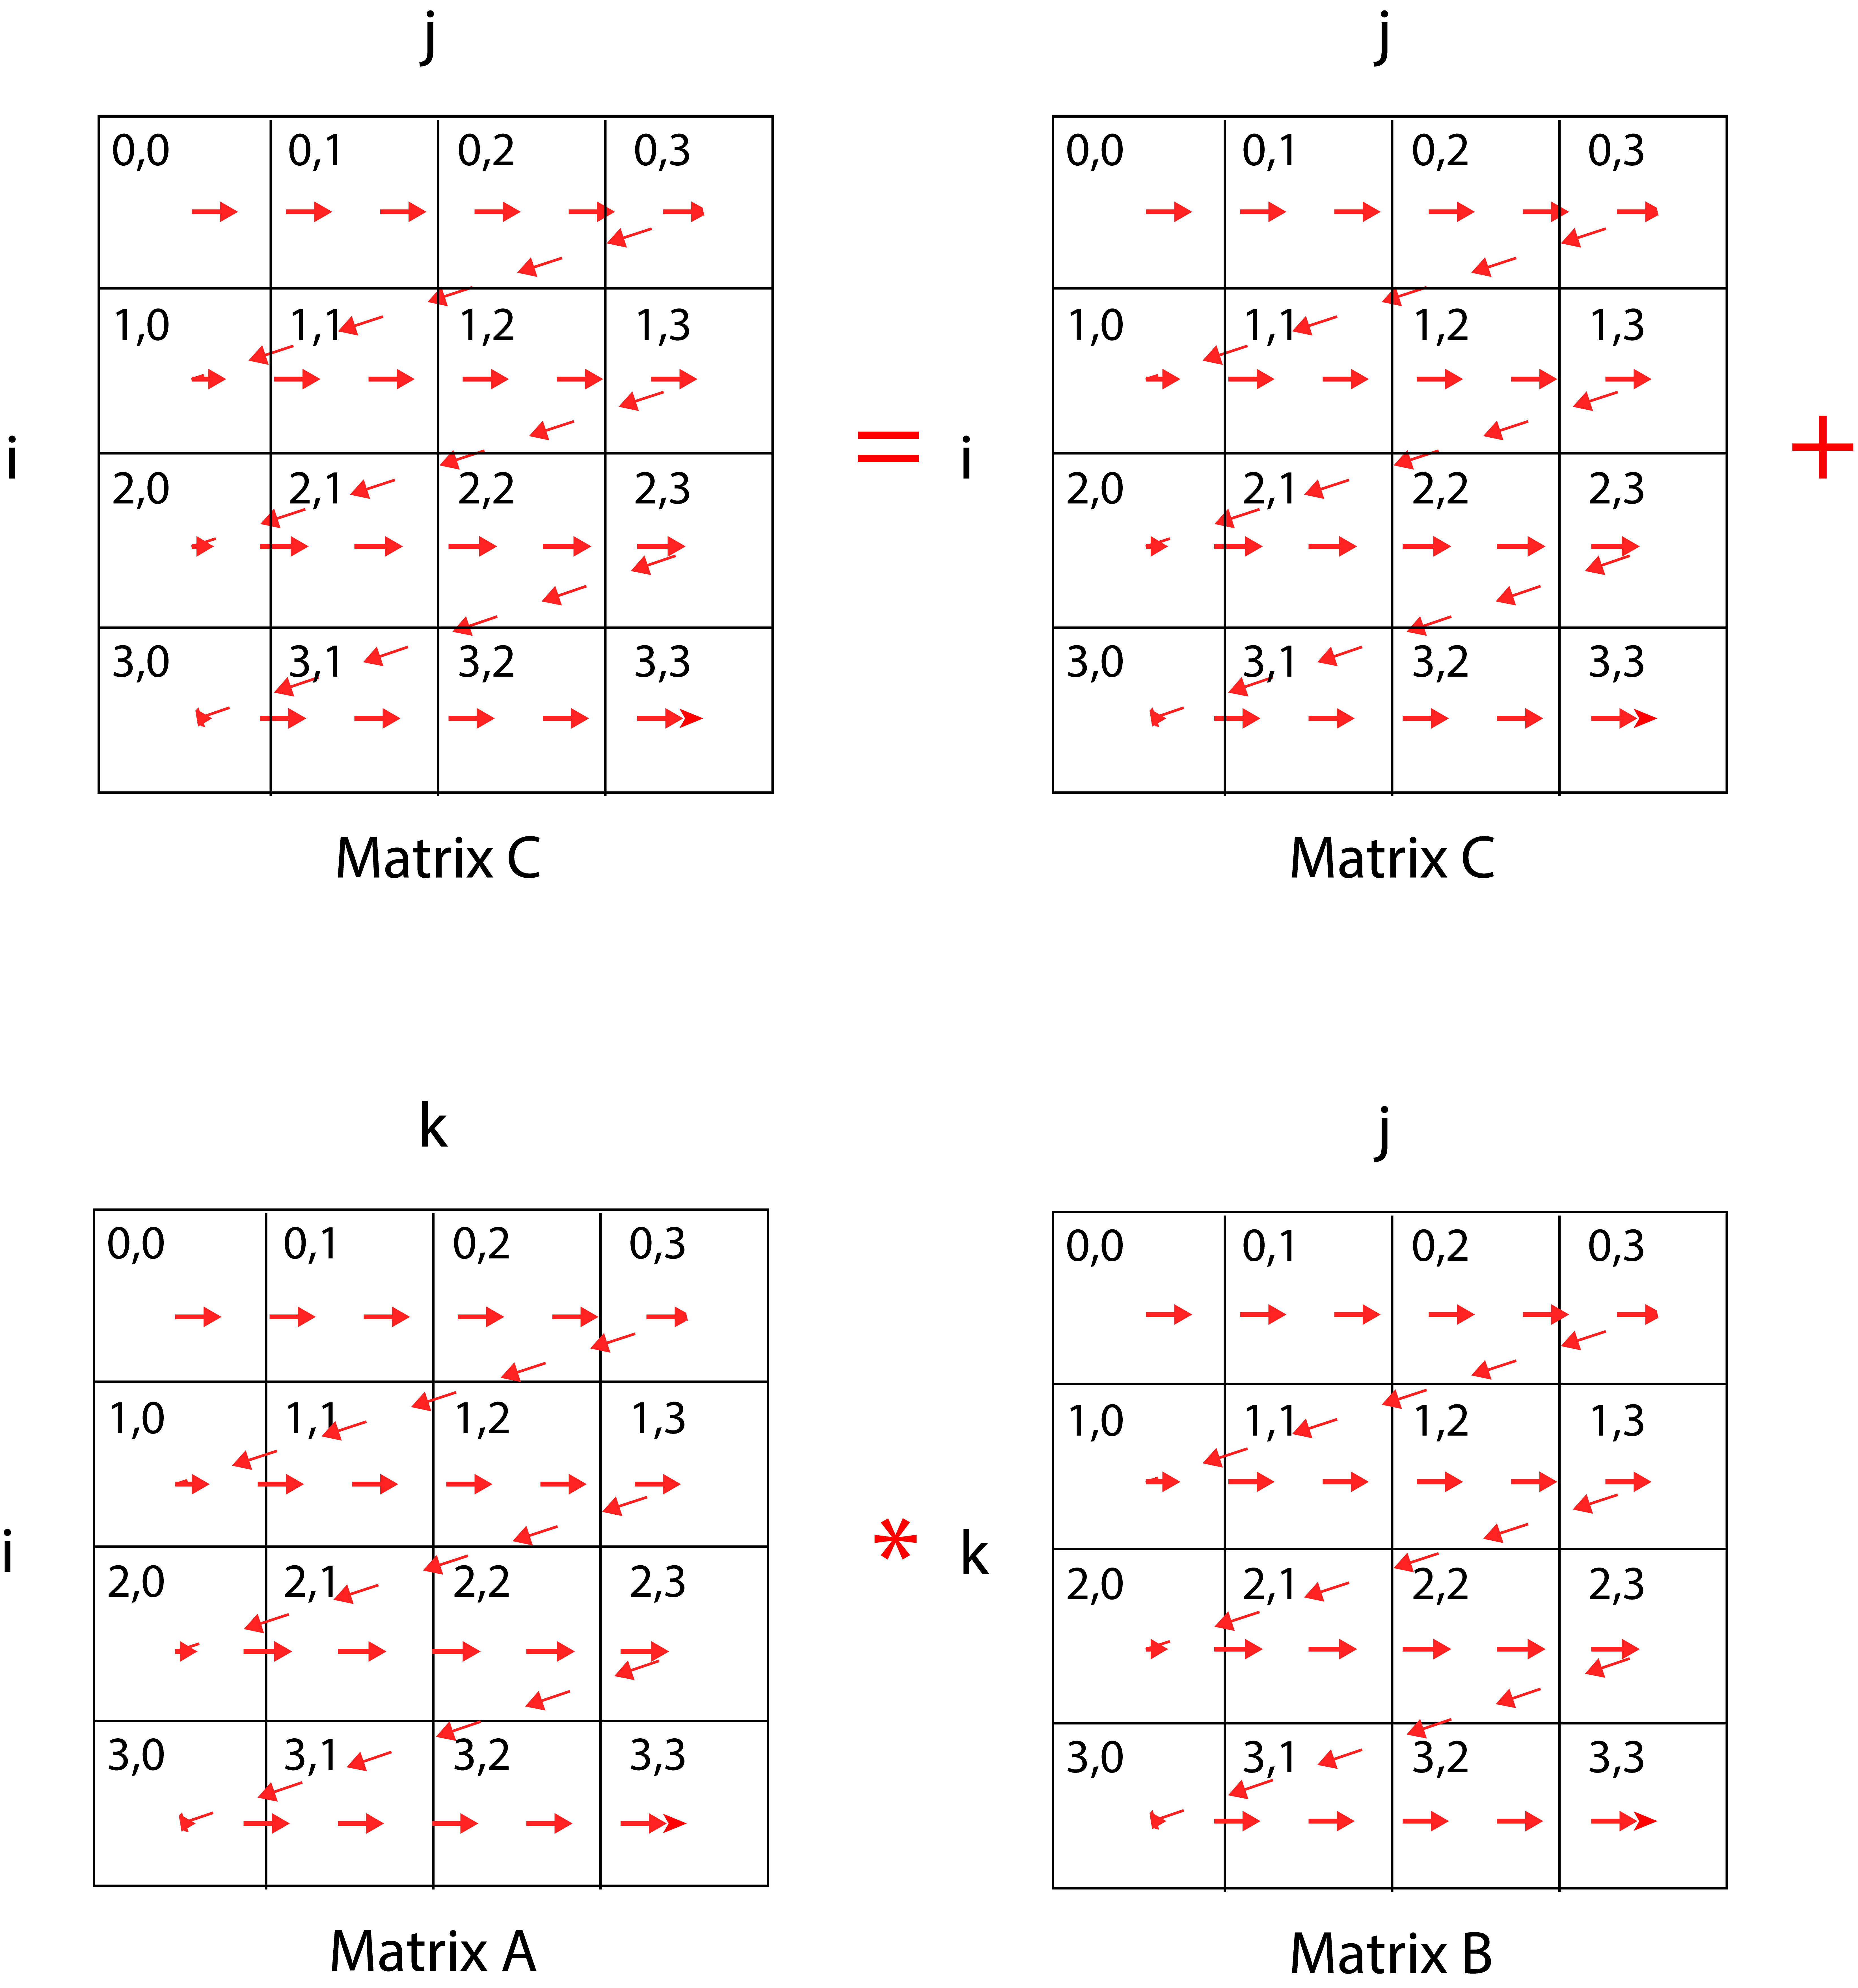
\includegraphics[width=0.75\columnwidth]{PNG/matrix_ikj_final.png}
\end{itemize}


A ordem dos ciclos I-J-K na versão naive resulta na constante invalidação das linhas de cache que correspondam a dados da matriz B. Ora, este problema irá acentuar-se em caso de necessidade de acesso à memórial principal, aumento a latência da recolha dos mesmos e provocando um atraso ainda mais visível quando comparada com a versão I-K-J.\par 


A seguinte tabela resume vários contadores de performance para as duas versões do kernel -- naive e interchange, para o dataset menor em estudo:


  \begin{table}[H]
  \caption{Performance events (naive vs. interchange) para o nó compute-431}
  \label{table:search_events}
  \centering
  \begin{tabular}{ | l | r | r |   }

  \hline
  \# EVENT NAME	 & NAIVE  & INTERCHANGE \\ \hline 
  cpu-cycles  & 535187277  & 399561216         \\ \hline       
  instructions &       1044692763 &      1152237507      \\ \hline
  cache-references &      8196140 &    429971      \\ \hline
  cache-misses     &    36522 &     43034      \\ \hline
  branch-instructions & 126101720 & 132065934      \\ \hline
  branch-misses     &   258384 &  249858      \\ \hline
  bus-cycles       &       0 &    0      \\ \hline
   L1-dcache-loads  &  246027409 & 253077242     \\ \hline
 L1-dcache-load-misses & 56436199 & 7577858   \\ \hline
  L1-dcache-stores   &  9973628 & 128034804     \\ \hline
  L1-dcache-store-misses & 322982 &  106020     \\ \hline
  LLC-loads           &    7391770 & 262810     \\ \hline
  LLC-load-misses      &  2671 &  1001     \\ \hline
  LLC-stores          &  218407 & 69369     \\ \hline
  LLC-store-misses    &   18512 &    0     \\ \hline
  dTLB-load-misses    &   2239 & 950     \\ \hline
  dTLB-store-misses   &    446 &  9     \\ \hline
  iTLB-load-misses   &   0 &   0     \\ \hline
  branch-loads   & 129163483 & 129898962  \\ \hline    
  branch-load-misses &  5688441 & 5560030      \\ \hline
  \end{tabular}
  \end{table}
  

Da análise da tabela   \ref{table:search_events} podemos confirmar que:

\begin{itemize}
\item O número de CPU cycles é menor para a versão interchange, reflectindo-se num menor tempo de solução.
\item O número de instruções é aproximadamente o mesmo dado para este dataset a invalidação dos dados não ser reflectida em leitura da memória principal mas apenas da LLCACHE (mais à frente neste relatório iremos analisar a influência da leitura da memória principal no tempo de execução).
\item O número de "cache-references" é muito maior para o caso naive (tal com esperado pela invalidação dos dados de matrizes).
\item O número de LLC loads é também muito maior para o caso naive (pela razão enumerada anteriormente).
\end{itemize}
Podemos então concluir que é este problema de padrão de acesso aos dados que resulta na degradação de performance da versão naive quando comparada com a versão interchange.\par 
Analisemos agora as métricas compostas, obtidas com base nos valores apresentados:


  \begin{table}[H]
  \caption{Performance rates (naive vs. interchange) para o nó compute-431}
  \label{table:search_rates}
  \centering
  \begin{tabular}{ | l | r | r |   }

  \hline
  RATIO OR RATE		 & NAIVE  & INTERCHANGE \\ \hline 
  Elapsed time (seconds) & 0.2041 & 0.1597   \\ \hline      
  
  Instructions per cycle  & 1.95  IPC & 2.88 IPC       \\ \hline      
  % Instructions per cycle	instructions / cycles
    % 1044692763 / 500890840 = 2,085
  % 1152237507 / 399561216 = 2,8837
  
          
  
  
  L1 cache miss ratio	  & 22,9389 \%   &     2,9942 \%    \\ \hline      
  % L1 cache miss ratio	L1-dcache-loads / L1-dcache-load-misses
  % 246027409 / 56436199  = 4,3593
  % 56436199 /  246027409 * 100 = 22,938988477
   % 253077242 / 7577858   = 33,3969
   
      % 7577858 / 253077242 * 100   = 2,9942866218

  L1 cache miss rate PTI &  54,0218 &     6,5766    \\ \hline     
  %L1 cache miss rate PTI 	L1-dcache-load-misses / (instructions / 1000)
     % 56436199 / ( 1044692763 / 1000)  = 54,0218
          %  (( 1044692763 / 1000)  / 56436199 ) *100 = 

   %  7577858 / ( 1152237507 / 1000)  = 6,5766
   
    L3 cache miss ratio	  & 0,0361 \%   &     0,3808 \%   \\ \hline      
  % L3 cache miss ratio	LLC-loads / LLC-load-misses
  % 7391770 / 2671  = 4,3593
    % (2671 / 7391770) * 100 = 0,0361

  % (1001 / 262810) * 100 = 0,3808
   % 1001 / 262810    = 33,3969
   
  
  Data TLB miss ratio	 &    0,00027 &   0,0022     \\ \hline      
  % Data TLB miss ratio	dTLB-load-misses / cache-references
  % 2239 / 8196140  = 0,00027
   %  950 / 429971  = 0,0008
   
  Data TLB miss rate PTI	 &   0,0021 &   0,0008    \\ \hline      
  % Data TLB miss rate PTI	dTLB-load-misses / (instructions / 1000)
   % 2239 / ( 1044692763 / 1000)  = 0,0021
   %  950 / ( 1152237507 / 1000)  = 0,0008
  
  Branch mispredict ratio	 & 0,002   &     0,0019  \\ \hline      
  % Branch mispredict ratio	branch-misses / branch-instructions
  % 258384 /  126101720 = 0,002
    % 249858 /  132065934 = 0,0019

  
  Branch mispredict rate PTI	 &  0,2473   &   0,2168    \\ \hline          
  % Branch mispredict rate PTI	branch-misses / (instructions / 1000)
  % 258384 / ( 1044692763 / 1000)  = 0,2473
   %  249858 / ( 1152237507 / 1000)  = 0,2168
   
     \end{tabular}
  \end{table}
  
A degradação de performance das versões, para o caso do dataset menor, não é traduzida numa exponenciação dos tempos totais para a solução, muito devido aos dados  apesar de estarem a ser acedidos de forma ineficiente, manterem-se contidos na LLCACHE. Focaremos a nossa análise doravante no dataset maior.\par 




    
  
  \section{Parte 3 }

\subsection{Período de amostragem e frequência de amostragem}

Dado que pretendemos encontrar os hotspots de ambas as versões, iremos usar a amostragem baseada em cpu-cycles. Desta forma, porções da aplicação que consumam mais tempo terão um maior número de amostras registadas. No entanto, este tipo de amostragem tem um preço -- pode ser demasiado pesada na avaliação de desempenho da aplicação. \par 

Temos que ter em conta que cada máquina tem um número de contadores máximos e fixados a certo tipo de eventos específicos. Ora, quando requeremos um grande número de eventos no profiling, é necessária a recorrência a multiplexagem, que gasta tempo de computação. Essa mesma multiplexagem poderá ter um peso demasiado elevado na avaliação de desempenho.\par 


Analisemos o tempo que demoram as versões large\_naive e large\_interchange sem qualquer tipo de ferramenta de amostragem por forma a podermos validar os resultados da avaliação de desempenho futura. Denote que por forma a validar os resultados foram realizadas 50 medições, sendo o valor apresentado o K Best (sendo K = 3) :

  \begin{table}[H]
  \label{table:base_rates}
  \centering
 \begin{tabular}{ | l | r | r |   }

  \hline
  EVENT NAME	 & L. NAIVE  & L. INTERCHANGE \\ \hline 
   Elapsed time & & \\ (seconds) & 10.43 & 65.61  \\ \hline    
  \end{tabular}
  \end{table}

Temos portanto agora uma base de referência também para estas versões que recorrem ao maior dataset em estudo. Voltemos portanto ao profilling das versões com os maiores datasets.\par 




Da análise de execução para as versões large\_naive e large\_interchange, foi produzida a seguinte tabela, que resume vários contadores de performance para as duas versões do kernel, para o dataset maior em estudo:

 \begin{table}[H]
  \caption{Performance events (naive vs. interchange) para o nó compute-431}
  \label{table:search_events_large}
  \centering
  \begin{tabular}{ | l | r | r |   }

  \hline
  \# EVENT NAME	 & NAIVE  & INTERCHANGE \\ \hline 
   Elapsed time & &  \\ \hline    
  instructions	& 38376000000 &  41776400000 \\ \hline    
cycles	& 78390700000 &  12384800000 \\ \hline    
cache-references	& 4744200000 &  14400000 \\ \hline    
cache-misses	&  4008300000 &  11200000 \\ \hline    
LLC-loads	& 4815000000  &  14800000 \\ \hline    
LLC-load-misses	& 4073600000 & 14400000  \\ \hline    
dTLB-load-misses & 1100000	& 100000  \\ \hline    
branches	& 3923900000 & 3847500000  \\ \hline    
branch-misses	&  2200000 &  1900000 \\ \hline    

  \end{tabular}
  \end{table}

\subsection{Análise comparativa do número de amostras por evento de hardware para as versões large\_naive e large\_interchange}




 \begin{table}[H]
  \caption{Sampling mode: large\_naive vs. large\_interchange
 para o nó compute-431}
  \label{table:search_sampling}
  \centering
  \begin{tabular}{ | l | r | r |   }

  \hline
  \# EVENT NAME	 & NAIVE  & INTERCHANGE \\ \hline   
  Elapsed time & &  \\ \hline    
  instructions & 383K samples	& 417K samples  \\ \hline    
cycles	& 783K  samples &  123K samples  \\ \hline    
cache-references &	47K samples & 144 samples   \\ \hline    
cache-misses & 40K samples	& 112 samples \\ \hline    
LLC-loads	 &  48K samples &  148 samples \\ \hline    
LLC-load-misses	& 40K samples & 144 samples  \\ \hline    
dTLB-load-misses	& 11 samples & 1 samples \\ \hline    
branches	&  39K samples &  38K samples \\ \hline    
branch-misses	& 22 samples & 19 samples \\ \hline    
   \end{tabular}
  \end{table}



  \section{Conclusão}






  % conference papers do not normally have an appendix



  % use section* for acknowledgment
  %\ifCLASSOPTIONcompsoc
  % The Computer Society usually uses the plural form
  % \section*{Acknowledgments}
  %\else
  % regular IEEE prefers the singular form
  %\section*{Acknowledgment}
  %\fi


  %The authors would like to thank...





  % trigger a \newpage just before the given reference
  % number - used to balance the columns on the last page
  % adjust value as needed - may need to be readjusted if
  % the document is modified later
  %\IEEEtriggeratref{8}
  % The "triggered" command can be changed if desired:
  %\IEEEtriggercmd{\enlargethispage{-5in}}

  % references section

  % can use a bibliography generated by BibTeX as a .bbl file
  % BibTeX documentation can be easily obtained at:
  % http://mirror.ctan.org/biblio/bibtex/contrib/doc/
  % The IEEEtran BibTeX style support page is at:
  % http://www.michaelshell.org/tex/ieeetran/bibtex/
  %\bibliographystyle{IEEEtran}
% argument is your BibTeX string definitions and bibliography database(s)
  %\bibliography{IEEEabrv,../bib/paper}
  %
  % <OR> manually copy in the resultant .bbl file
  % set second argument of \begin to the number of references
% (used to reserve space for the reference number labels box)


  %\begin{thebibliography}{1}

  %\%bibitem{nas}
  %NAS Parallel Benchmarks, \url{http://www.nas.nasa.gov/publications/npb.html}

  %\end{thebibliography}

  %\appendix 


  % that's all folks
  
  
  
\lstinputlisting[style=command]{../12_command.txt} %input de um ficheiro
\lstinputlisting[language=C]{../12_event_list.txt} %input de um ficheiro

\lstinputlisting[style=command]{../13_command.txt} %input de um ficheiro
\lstinputlisting[language=C]{../13_perf_list_wc.txt} %input de um ficheiro

\lstinputlisting[style=command]{../14_command.txt} %input de um ficheiro
\lstinputlisting[language=C]{../14_insns_per_cycle.txt} %input de um ficheiro

\lstinputlisting[style=command]{../15_command_naive.txt} %input de um ficheiro
\lstinputlisting[language=C]{../15_perf_events_table_naive.txt} %input de um ficheiro

\lstinputlisting[style=command]{../15_command_interchange.txt} %input de um ficheiro
\lstinputlisting[language=C]{../15_perf_events_table_interchange.txt} %input de um ficheiro




  \end{document}


